%!TEX root = ../report.tex

% 
% Architecture
% 

\section{Architecture}

There is a lack of refactoring tools for dynamic languages, and some dynamic languages such as Racket are good to start learning how to program.
The idea is to create a refactoring tool that would suit an unexperienced programmer that is starting to learn how to program. That is a tool that is simple to use and that the programmer is not afraid to use the refactoring tool.
Because of this concerns, the choice of IDE is important, and that is why the DrRacket IDE was chosen.

The idea is to create restructuring tool for DrRacket, DrRacket is an integrated development environment (IDE), that was formerly known as DrScheme. It is a simple IDE that was initially build for Racket programming language and it is aimed at inexperienced programmers. ({\bf Fig.~\ref{fig:DrRacketGui}}).
It was designed as a pedagogic environment \cite{drscheme_pegadogy} and it was used in many introductory programming courses in schools around the world. In addition to that DrRacket supports development and extension of other programming languages \cite{tobin2011languages} and recently it have an implementation of python. \cite{ramos2014implementation}

%it is not an intention to care about refactorings regardint meta-programming or reflection calls. Even the Static object oriented refactoring tools with all their refactoring operations, developers do not try to solve that problem.

Racket \footnote{http://racket-lang.org/} programming language is a dialect of lisp and a descendant of Scheme and support objects, types and laziness evaluation,
whereas Python is a very high-level programming language that supports the imperative, functional and object-oriented programming paradigms and is very popular in many areas.

Besides being a simple and a good IDE to learn how to program, DrRacket gives some functionalities that are helpful to the programmer of the refactoring tool. DrRacket knows all the bindings of each variable and represents that binding with arrows. Each arrow knows where is pointing to and where is the beginning of itself. This is rather helpful for the refactoring operations that need semantics, for example for the extract-function it makes it very easy to know what variables will be arguments of the extracted function and what variables are not needed to be passed as arguments.

DrRacket also have syntax objects, these objects have all the information regarding the syntactic information and their location. Basically they represent an AST annotated with the location of each object.

By having this features it is possible to create a tool that helps the unexperienced users and it is useful for more experienced users.









%DrRacket Image
\begin{figure}[htbp]
	\centering
	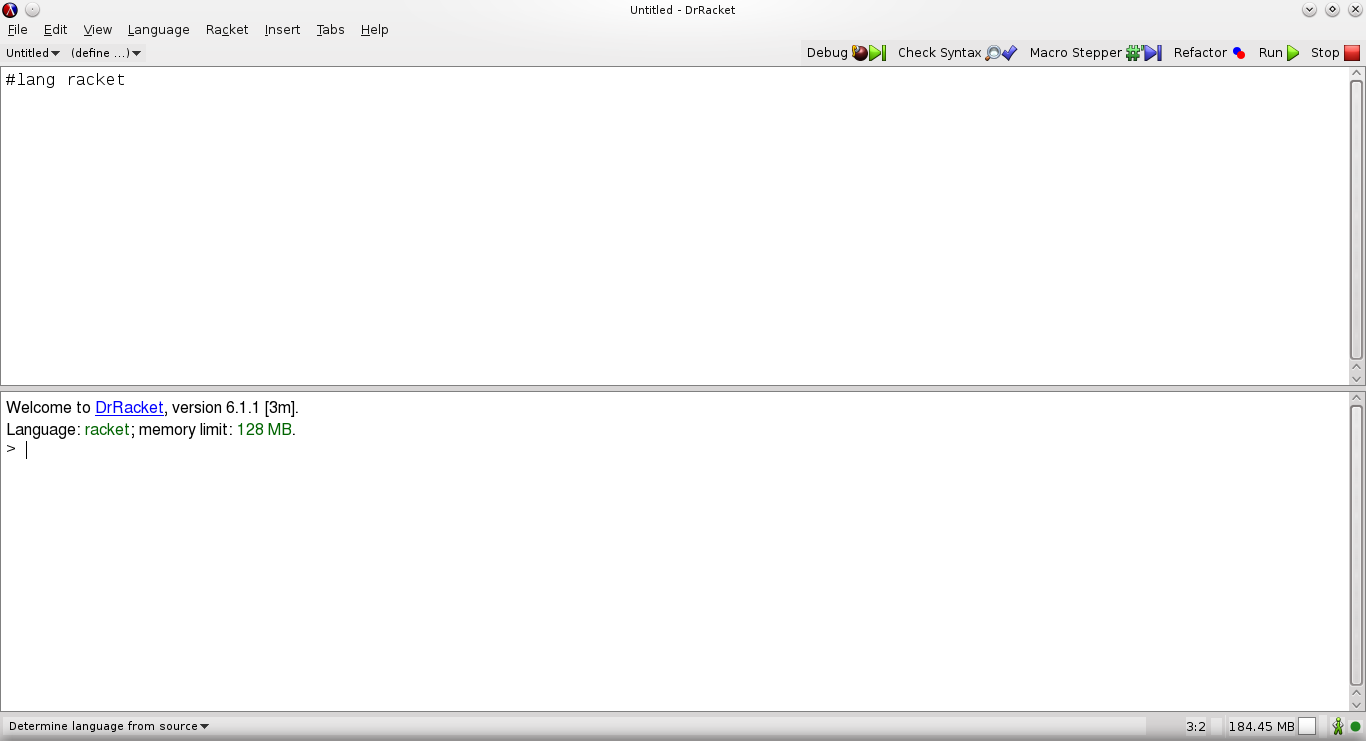
\includegraphics[width=0.6\textwidth]{img/DrRacketGui.png}
	\caption{DrRacket Graphical user interface}
	\label{fig:DrRacketGui}
\end{figure}